% This file is isea.tex.  It contains the formatting instructions for and acts as a template for submissions to ISEA 2015.  It is based on the ICCC  formats and instructions.  It uses the files isea.sty, isea.bst and isea.bib, the first two of which also borrow from AAAI IJCAI formats and instructions.
% Modified from ICCC.tex by B. Bogart

\documentclass[letterpaper]{article}
\usepackage{isea}
\usepackage[pdftex]{graphicx}
\usepackage{times}
\usepackage{helvet}
\usepackage{courier}
\usepackage[numbers]{natbib}
\pdfinfo{
/Title (Scaling with multiple network namespaces in a single application)
/Author (PJ Waskiewicz)}
% The file isea.sty is the style file for ISEA 2015 proceedings.
%
\title{Scaling With Multiple Network Namespaces in a Single Application}
\author{PJ Waskiewicz\\
Principal Engineer at NetApp\\
Portland, OR, USA\\
pj.waskiewicz@netapp.com\\
\newline
\newline
}
\setcounter{secnumdepth}{0}

\begin{document} 
\maketitle
\begin{abstract}
Namespaces and containers seem to be the rage today, but it’s not typical for large applications to use them directly. Rather, applications rely on frameworks such as LXC and/or Docker to manage the containers they run in.

This paper will focus on how a large application can utilize the network namespace framework, and how it can use large numbers of namespaces to partition up the underlying network infrastructure within the application. An overview of parts of the application architecture using the namespaces will be covered, showing the use cases driving the need for namespaces. Lessons learned around scalability and performance bottlenecks in the kernel will be shared.

Ultimately this paper will propose further improvements to the namespace framework for better programmatic management of namespaces within the kernel from userspace, as well as attention to increased scalability and efficiency of networking within the namespaces.
\end{abstract}

\section{Keywords}

networking, kernel, containers, namespaces, scaling, cloud

\section{Introduction}
The ongoing evolution of the datacenter towards cloud-based infrastructure continues to present interesting challenges to existing applications. These existing solutions, e.g. storage appliances, work to serve multiple tenants within a computing domain. However, when the infrastructure around these solutions evolves into a cloud-based, partitioned environment, these solutions must also evolve.

When an application has core logic that needs to span multiple, separate network environments, it must become container/network-namespace aware. The Linux kernel exposes an API to create and manage network namespaces within an application. This paper will focus on this API for the following:
\begin{itemize}
\item How to create and manage the lifecycle of a network namespace within a complex application
\item How to track and process multiple network connections across multiple network namespaces in an efficient and scalable manner
\item What limitations exist in this API that makes lifecycle management a challenge, along with proposals on how to improve the API for better lifecycle management
\item Scalability issues encountered, how these were addressed, and proposals around scalability testing to prevent regressions
\end{itemize}

\section{The Need For Multiple Namespaces}
\begin{figure}[h]
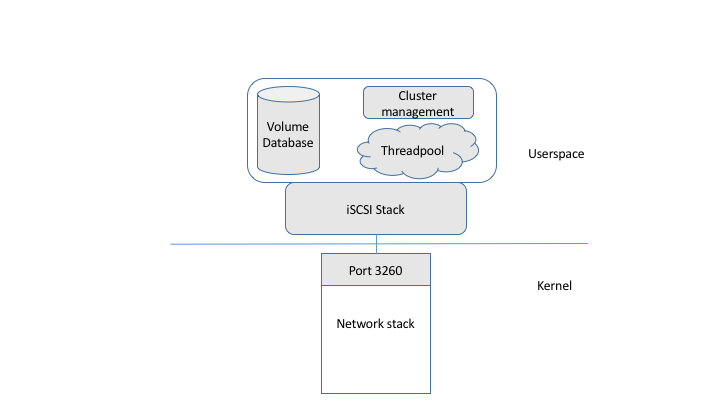
\includegraphics[width=3.31in]{standard-app-overview.png}
\caption{High-level architecture of application.}
\end{figure}

\subsection{Section Headings}

Print section headings centered, in 12-point bold type in the style shown in these instructions. Your body text should be 10 point, justified, single space. Do not number sections.

\subsubsection{Subsection Headings}

Print subsection headings left justified, in 11-point bold type and mixed case (nouns, pronouns, and verbs are capitalized). They should be flush left. Your text should be 10 point, justified, single space. Do not number subsections.

\section{Acknowledgments}
We would like to acknowledge the engineers who contributed to this network namespace application design: Joe Roback, Carl Seelye, Tom Distler, Jared Cantwell, and Marshall McMullen.

We would also like to acknowledge the Netdev1.2 selection committee for inviting us to submit and present this paper.

\bibliographystyle{pj-netdev-1.2}
\bibliography{pj-netdev-1.2}

\section{Author Biography}
PJ Waskiewicz is a Principal Software Engineer at NetApp in the SolidFire division. Prior to SolidFire/NetApp, PJ worked for many years as a network kernel engineer and device driver developer in the Networking Division of Intel. There he maintained and helped create the igb, ixgbe, and i40e wired Ethernet network drivers. He also worked in Intel's Open Source Technology Center on the x86 kernel tree, enabling advanced features in the Broadwell and Skylake microarchitectures.

\end{document}
